
\section{Ultrasound Design Gallery}\label{section:usdg}

In this section, we introduce the \usdg.
The \usdg~is primarily based on two components: a user interface (\cref{section:ui}) and an algorithm for learning (\cref{section:gp}) and optimizing the sonographer's preference (\cref{section:bo}).

\subsection{User Interface of the \usdg}\label{section:ui}
\subsubsection{Design Galleries}
Humans are notorious for not being able to quantify their preference in an \textit{absolute scale}.
In comparison, when asked to \textit{relatively compare} different candidates, humans are more capable of telling which one they liked over the others~\cite{10.2307/27821441, NIPS2007_b6a1085a}.
The \textit{Design Gallery interface}~\cite{10.1145/258734.258887} builds upon this principle.
It proposes multiple different \textit{candidates} and lets the user choose which one he preferred over the others.
While the original Design Gallery and the variant proposed by Brochu et al.~\cite{brochu_bayesian_2010} propose only a discrete set of candidates, Koyama \textit{et al.}~proposed design galleries that suggest a continuous set of candidates embedded on a 1D line~\cite{10.1145/3072959.3073598} and a 2D plane~\cite{koyama_sequential_2020}.
In our context, an important consideration is that medical ultrasound images are best presented in videos rather than still images.
In this case, presenting multiple videos on a 2D plane can be confusing.
Therefore, the Ultrasound Design Gallery is based on the 1D sequential line search scheme proposed by Koyama \textit{et al.}~\cite{10.1145/3072959.3073598}.

\subsubsection{Overview of the Ultrasound Design Gallery Interface}
%
\begin{figure}[h]
  \centering
  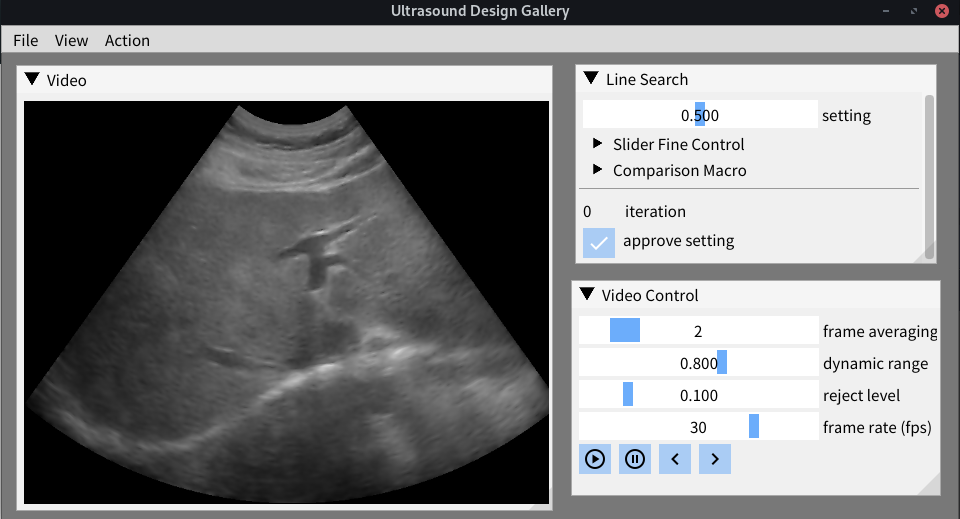
\includegraphics[scale=0.30]{figures/ui.png}
  \caption{User interface of the Ultrasound Design Gallery. We can see the \textbf{video (preview) window} (left), the \textbf{line search window} (top right), and the \textbf{video control window} (bottom right) }\label{fig:ui}
\end{figure}
%
The user interface of the Ultrasound Design Gallery is shown in~\cref{fig:ui}.
It comprises of three basic components:
    \vspace{0.05in}
\begin{enumerate}
  \item[\ding{228}] \textbf{Video (preview) window}: This window displays the image processed using the currently chosen image processing parameter setting.
    \vspace{0.05in}
  \item[\ding{228}] \textbf{Line search window}: This window contains the slider which is the 1D space where the image processing parameters are embedded.
    \vspace{0.05in}
  \item[\ding{228}] \textbf{Video control window}: This window provides basic controls of the image presentation such as dynamic range, frame rate, and the likes.
\end{enumerate}
The user is supposed to interact with the slider in~\textbf{video control window}, each slider position signifies a certain image processing parameter setting embedded on the 1D line.
The \textbf{video window} presents the image sequence processed with this setting in real time.
This process is illustrasted in~\cref{fig:interaction}
Note that the image processed and displayed through the \textbf{video window} is a pre-recorded sequence of ultrasound images.

\subsubsection{Interacting with the Ultrasound Design Gallery}
%
\begin{figure}[h]
  \centering
  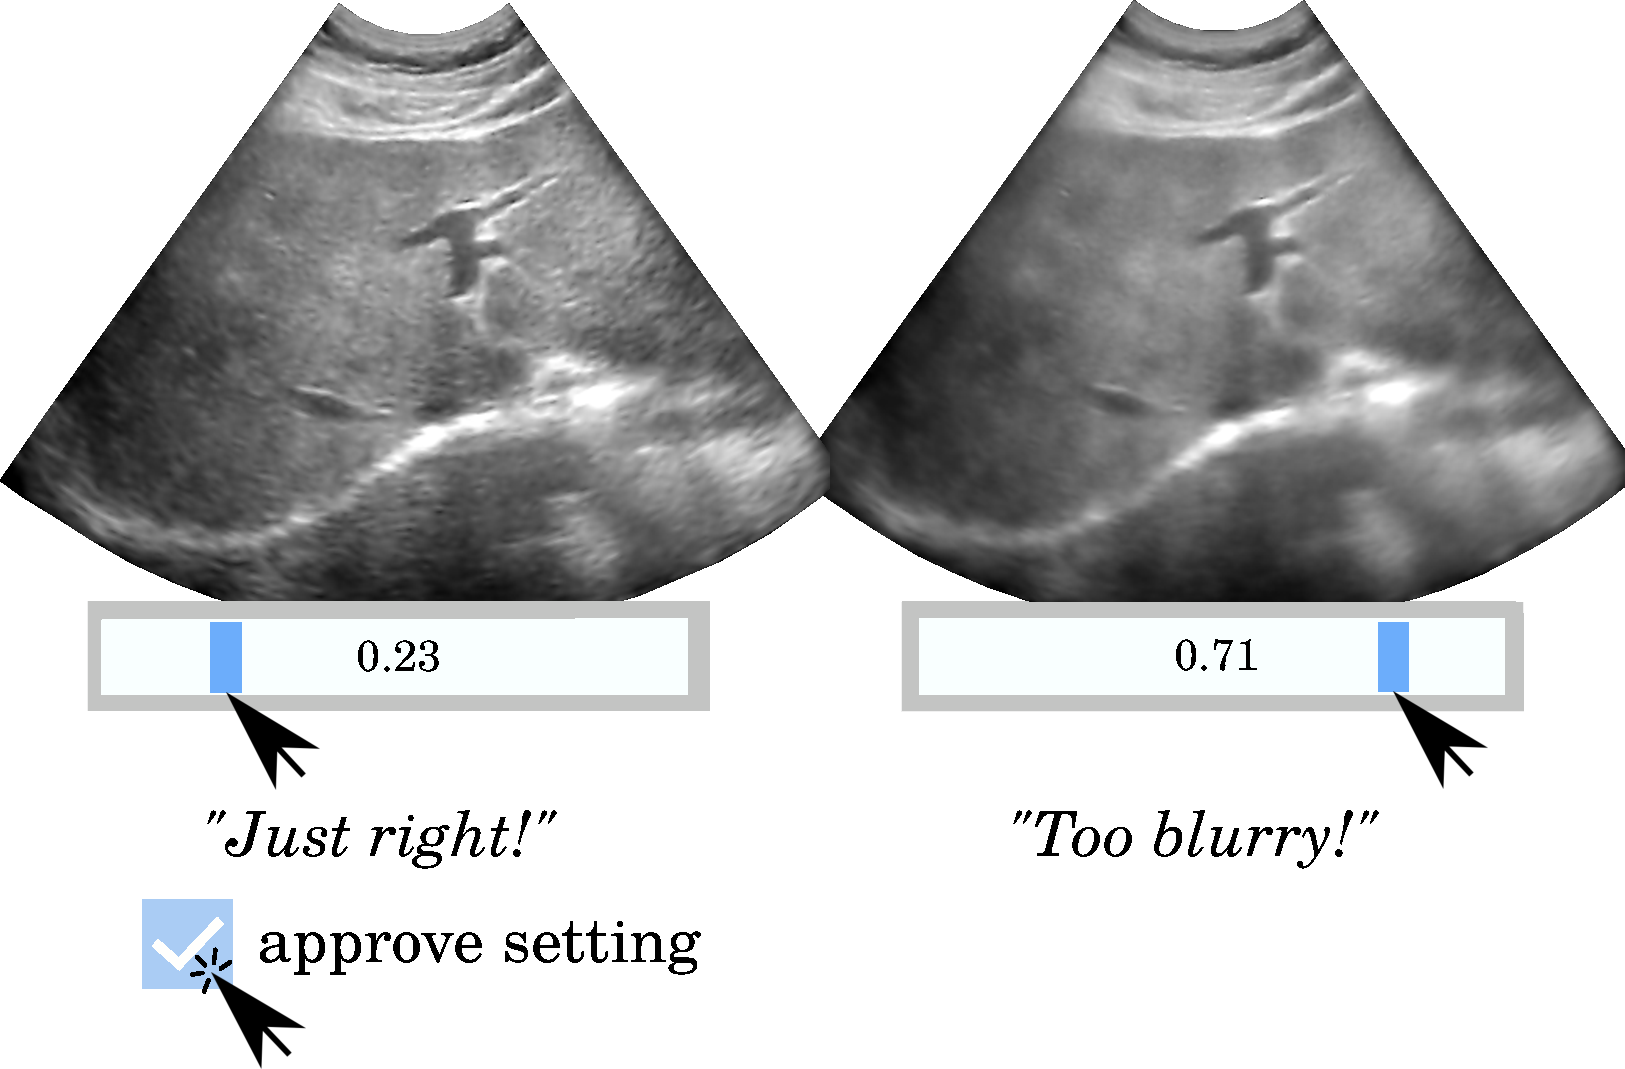
\includegraphics[scale=0.3]{figures/ui_interaction.pdf}
  \caption{Visualization of the interaction with the Ultrasound Design Gallery}\label{fig:interaction}
\end{figure}
%
The basic workflow of using the \usdg~is as follows:
\begin{enumerate}
\item[\ding{182}] The user is first presented with images processed using randomly sampled parameter settings.
\item[\ding{183}] The user compares the random settings embedded on the 1D line by interacting with the slider in the line search and approves the most preferred setting. This process is illustrated in~\cref{fig:interaction}.
\item[\ding{184}] The \usdg~records the choice and recommends a new set of parameter settings using Bayesian optimization, which is also embedded on a 1D line.
\item[\ding{185}] The user compares the recommeded settings by interacting with the slider as in step~\ding{183}.
\item[\ding{186}] Go back to step~\ding{184} until convergence.
\end{enumerate}

\begin{figure}[h]
  \centering
  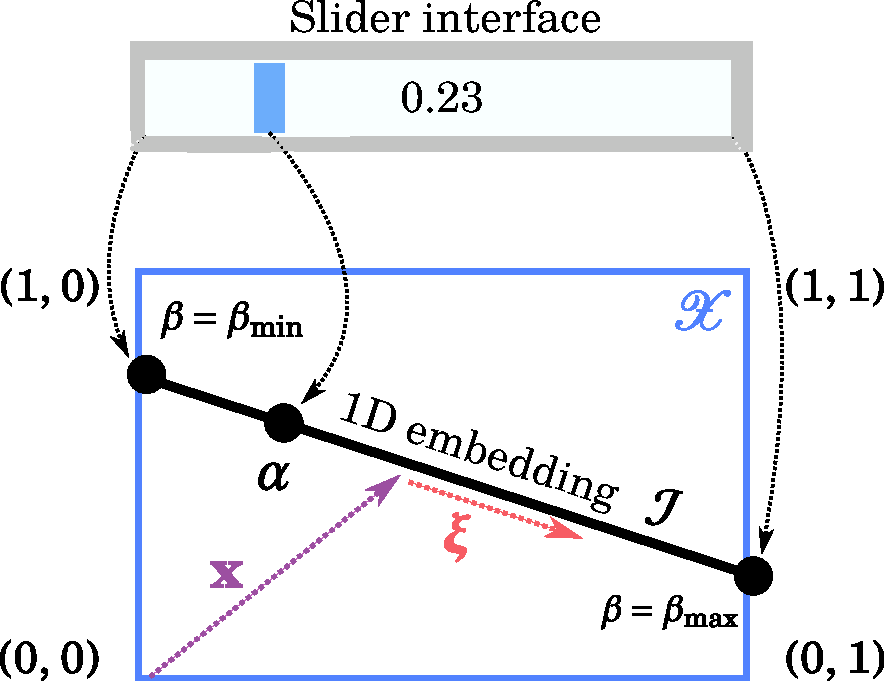
\includegraphics[scale=0.35]{figures/linesearch.pdf}
  \caption{Visualization of the relationship between the slider interface and the parameter space \(\mathcal{X}\).
    We show a two-dimensional parameter space \(\mathcal{X} = {[0, 1]}^2\) for illustration.
    The one dimensional projection is performed using the basis vector \(\vx\) and the direction vector \(\vxi\).
  }\label{fig:linesearch}
\end{figure}
%
Formally, the user is solving the line seach problem
\begin{align}
 \alpha = &\argmax_{ \beta }\; f\,(\beta\,\vxi + \vx) \\
 &\text{subject to}\;\; \beta_{\mathrm{min}} \leq \beta \leq \beta_{\mathrm{max}}
\end{align}
where \(f\) is the preference function of the user, \(\beta\) is a position on the 1D line, \(\vx\) and \(\vxi\) are the basis and direction of the 1D line, \(\mathcal{X}\) is the domain of all the parameter settings.
\(\beta_{\mathrm{min}}\) are \(\beta_{\mathrm{max}}\) are bounds that ensure that \(\beta\,\vxi + \vx  \in \mathrm{X}\).
The user choice minimizing \(\alpha\) is denoted as \(\alpha\).
A geometric illustration of the correspondance between the graphical interface and our mathematical notations is provided in~\cref{fig:linesearch}.

Our goal is to find the best parameter setting \(\vx^{*}\) that maximizes the user preference \(f\) given that the user successively solves this line search problem.

\subsection{Learning the Preference of Sonographers with Gaussian Processes}\label{section:gp}
\subsubsection{Probabilistic Model}
\paragraph{Gaussian Process Formulation}
Once the user has provided his feedback, we analyze it and suggest a new 1D embedding that potentially contains the optimal parameter setting \(\vx^{*}\).
At the \(t\)th iteration, the user feedback is represented by \(\vx_t\), \(\vxi_t\) which are the sufficient information about the 1D line, and the optimal position on the line \(\alpha_t\).
Analyzing this information is posed as a machine learning problem where we reconstruct \(f\) given the history of the user choices from 1 to \(t\), \(\mathcal{D}_t = \{\,(\vx_1, \vxi_1, \alpha_1), \ldots, (\vx_t, \vxi_t, \alpha_t)\,\}\).

For a datapoint \( (\vx_t, \vxi_t, \alpha_t) \), each point \(\beta\,\vx_t + \vxi_t\) on the line sastisfies
\begin{align}
f(\beta\,\vx_t + \vxi_t ) > f(\alpha\,\vx_t + \vxi_t) \;\;\text{for all}\;\; \beta \in [\beta_{\mathrm{min}}, \beta_{\mathrm{max}}]
\end{align}
Note that \(\beta_{\mathrm{min}}\) and \(\beta_{\mathrm{max}}\) are in fact dependent on \(\vx\), \(\vxi\).
For conciseness, we drop the dependence in our notation.
We formulate this setting into a latent Gaussian process model~\cite{rasmussen_gaussian_2006} described as follows:
\begin{align}
\epsilon_{\vf}           &\sim p\,(\epsilon_{\vf}) \\
\sigma                  &\sim p\,(\sigma) \\
\vf \mid \epsilon_{\vf}  &\sim \mathcal{GP}(0, \mK + \epsilon_{\vf}^2\mI) \\
  f(\alpha\,\vxi + \vx) > f(\beta_i \,\vxi + \vx) \mid \vf,\, \sigma
  &\sim p\,(\alpha,\, \beta_i,\, \vx,\,\vxi,\, \mid \epsilon,\, \vf). 
\end{align}
where \(\epsilon_{\vf}\) is the noise included in the preference evaluations, \(\sigma\) is the variance of the values of \(f\), \(\vf\) is the function represented as a vector in the Gaussian process, \(\mathcal{\mK}\) is 

\paragraph{Likelihood Function}
The most important component in our model is the likelihood function \(p\,(\alpha,\, \beta_i,\, \vx,\,\vxi,\, \mid \epsilon,\, \vf)\).
Since our 1D line contains an \textit{infinite} number of duels between each \(\beta\) and \(\alpha\), it is difficult to formulate a proper likelihood function.
The original sequential line search design galleriy discretized the 1D line and proposed a likelihood function based on the Bradley-Terry-Luce model~\cite{10.1145/3072959.3073598}.
Since the Bradley-Terry-Luce model assumes a discrete number of candidates, there is no reason to belive discretization is appropriate.
Instead, we take a much more principled approach by Mikkola \textit{et al.}~\cite{pmlr-v119-mikkola20a}.
In particular, Mikkola \textit{et al.} propose a likelihood function that can fully represent candidates embedded on a continuous space.

\begin{figure}[t]
  \removelatexerror
  \begin{algorithm2e}[H]
    \DontPrintSemicolon
    \SetAlgoLined
    \KwIn{Precomputed Cholesky decomposition of \(\mK\),
      convergence criterion, 
      gradient function of the likelihood \(\nabla_{\vf}\, p(\mathcal{D}\mid\vf)\),
      Hessian function of the joint \(\nabla^2_{\vf}\, p(\mathcal{D},\, \vf)\).
    }
    \KwOut{
      \(\vf_{t}\), \(\mW_t\).
    }
    \( \vf_1 \leftarrow \mathbf{0} \)\;
    \Repeat{ until convergence } {
      \(\valpha        \leftarrow \mK\backslash\vf_{t} \)\;
      \(\vg            \leftarrow \nabla_{\vf}\, p(\mathcal{D}\mid\vf)|_{\vf = \vf_t} - \valpha \)\;
      \(\mW_t          \leftarrow -  \nabla^2_{\vf}\, p(\mathcal{D},\, \vf) \)\;
      \(\mB           \leftarrow \mI + \mK \mW \)\;
      \(\mL_{\mB}, \mU_{\mB} \leftarrow \mathrm{lu}\,(\mB) \)\;
      \(\vp           \leftarrow \mL_{\mB} \backslash \mU_{\mB} \backslash \mK \vg \)\;
      \(\vf_{t+1}      \leftarrow \vf_t + \eta \, \vp \)\;
      \(t \leftarrow t + 1\)\;
    }
    \caption{Newton's Method for Laplace's Approximation}\label{alg:newton}
  \end{algorithm2e}
\end{figure}
%
\subsubsection{Inference with Laplace's Approximation}
We approximate the posterior \(p\,(\vf\,|\,\vtheta,\, \mathcal{D})\) with Laplace's approximation~\cite{williams_bayesian_1998}.
Laplace's approximation performs a second order Taylor expansion around the maximum of the posterior such that
\begin{align}
q\,(\vf) = \mathcal{N}\left(\vf;\, \vf^*,\, {(\mK^{-1} + \mW)}^{-1}\right) \approx p\,(\vf \mid \vtheta,\, \mathcal{D})
\end{align}
where \(\vf^*\) is the maximum a-posteriori estimate such that \(\nabla_{\vf}\, p\,(\mathcal{D},\, \vf)|_{\vf = \vf^*} = 0\), \(\mW = -\nabla^2_{\vf}\, p\,(\mathcal{D},\,\vf)|_{\vf=\vf^*} \) is the negative Hessian of the likelihood at \(\vf^*\), and \(\mK\) is the covariance matrix.
In general, \(\mH\), the Hessian of \(p\,(\mathcal{D},\vf)\) turns out structured.
This allows efficient implementations of Newton's method for finding \(\vf^*\).
For example,~\cite{rasmussen_gaussian_2006} discusses cases where \(\mH\) is diagonal or block-diagonal.
Unfortunately, in our case, the structure of \(\mH\) is neither.
We thus provide a different implementation of Newton's iteration that uses the identities
\begin{align}
  {\big(\mK^{-1} + \mW\big)}^{-1}
  &= {\Big(\mK^{-1} \big(\mI + \mK \mW \big)\Big)}^{-1} \\
  &= {{\big(\mI + \mK \mW \big)}^{-1} \mK} \\
  &= \mB^{-1} \mK \\
  &= \mU_{\mB}^{-1} \, \mL_{\mB}^{-1} \, \mK \label{eq:BinvK}
\;.
\end{align}
where \cref{eq:BinvK} is computed using the LU decomposition of \(\mB\) and back-substitution.
A detailed illustration is provided in~\cref{alg:newton} where \(\vp\) is the Newton direction, the stepsize \(\eta\) is found using backtracking line search with Armijo's condition~\cite{nocedal_numerical_2006}.

\subsubsection{Predictive Distribution}
For prediction, we use a formulation of \({\big(\mK^{-1} + \mW\big)}^{-1}\) different from~\cref{eq:BinvK}.
This is because the variance prediction \(\sigma^2(\vx)\) which requires to compute a inverse quadratic term \(\mK^{\top}(\vx) {\big(\mK^{-1} + \mW\big)}^{-1} \vk(\vx)\), which can be efficiently computed when a Cholesky decomposition of \(\mL_{\mathcal{L}} \, \mL^{-1}_{\mathcal{L}}  = {\big(\mK^{-1} + \mW\big)}\) is available.
The formulation of~\cref{eq:BinvK} does not directly provide a closed form expression for the Cholesky.
We thus use the indentities
\begin{align}
  {\big(\mK^{-1} + \mW\big)}^{-1}
  &= { \Big({\big(\mL\,\mL^{\top}\big)}^{-1} + \mW \Big) }^{-1} \label{eq:Kcholid}  \\
  &= { \big(\mL^{-\top}\,\mL^{-1} + \mW \big) }^{-1}  \\
  &= { \Big( \mL^{-\top}\,\big(\mI + \mL^{\top}\,\mW\,\mL \big)\,\mL^{-1} \Big) }^{-1}  \\
  &= \mL\,{\big(\mI + \mL^{\top}\,\mW\,\mL \big)}^{-1}\,\mL^{\top}  \\
  &= \mL\, \mC^{-1} \,\mL^{\top}  \\
  &= \big( \mL\, \mL_{\mC}^{-1} \big)\, {\big( \mL\, \mL_{\mC}^{-1} \big)}^{\top} \label{eq:Ccholid} \\
  &= \mL_{\mathcal{L}} \, { \mL_{\mathcal{L}} }^{\top}
\end{align}
where~\cref{eq:Kcholid} uses the precomputed Cholesky decomposition of \(\mK\) and~\cref{eq:Ccholid} requires the Cholesky decomposition of \(\mC = \mI + \mL^{\top}\,\mW\,\mL\).

The GP prediction using \(q\,(\vf)\) are computed as
\begin{align}
  \mu\,(\vx)
  &= {\vk(\vx)}^{\top} \mK^{-1} \, \vf^*  \\
  \sigma^2\,(\vx)
  &= k(\vx, \vx) - \vk^{\top}(\vx) \, {(\mK^{-1} + \mW)}^{-1} \, \vk(\vx) \\
  &= k(\vx, \vx) - {\big( \mL_{\mathcal{L}} \vk(\vx) \big)}^2
\end{align}

\subsubsection{Hyperparameter Treatment}
While previous works observed that the full Bayesian approach improves performance~\cite{henrandez-lobato_predictive_2014, snoek_practical_2012}, recent experimental results suggest that such performance improvement may not be significant~\cite{ath_bayesian_2021}.
In our case, the exact marginal likelihood is not available.
Thus, full Bayesian inference requires pseudo-marginal MCMC~\cite{filippone_pseudomarginal_2014, pmlr-v51-murray16} methods, which suffer from low statistical effieciency for high-dimensions.
Also, the real-time nature of our application makes the use of these methods very delicate in terms of computational efficiency and robustness.
We experimented with full Bayesian inference using pseudo-marginal slice-sampling~\cite{pmlr-v51-murray16} and concluded that it is not worth the computational cost.

Some theoretical~\cite{berkenkamp_noregret_2019} and practical~\cite{wang_adaptive_2013} works have suggested that expert tuned hyperparameters achieve better performance than full Bayesian treatments.

%% \paragraph{Pseudo-Marginal MCMC}
%% Using our approximation \(q\,(\vf)\), we use  for sampling both \(\vf\) and \(\vtheta\) from the posterior.
%% The marignal likelihood is approximated using importance sampling such that
%% \begin{align}
%%   \tilde{p}\,(\mathcal{D}\mid\theta)
%%   &= \int p\,(\mathcal{D}\mid\vf)\,p\,(\vf\mid\vtheta) d\vf \\
%%   &\approx \frac{1}{N_{\mathrm{pm}}} \sum^{N_{\mathrm{pm}}}_{i=1} \frac{p\,(\mathcal{D}\mid\vf_i)\,p\,(\vf_i\mid\vtheta)}{q\,(\vf_i)}
%% \end{align}
%% where \(\vf_i\) are samples from \(q\,(\vf)\) and \(N_{\mathrm{pm}}\) is the number of samples.
%% For simplicity, we use the maximum a-posteriori estimate \(\vf^*\).

%% For sampling \(\theta\) and \(\sigma\), we use elliptical slice sampling~\cite{murray_elliptical_2010}.
%% To resolve this problem, Murray \& Graham propose pseudo-marginal slice sampling~\cite{}.

%% Using the ARD hyperparameters alone for sensitivity analysis results is not very effective~\cite{pmlr-v89-paananen19a}.
%% Also, the non-identifiability of ARD hyperparameters complicates their statistical analysis~\cite{zhang_inconsistent_2004a}.
%% ARD is severely affected by dimensionality.
%% This manifests as low acceptance rates in MCMC procedures~\cite{filippone_pseudomarginal_2014}.

\subsection{Optimizing \User~Preference with Preferential Bayesian Optimization}\label{section:bo}

\begin{align}
 &\minimize_{\vx,\, \vxi}\;\; a\,(\vx, \vxi \mid \mathcal{D}) \\
 &\text{subject to}\;\; \vx \in \mathcal{X},\; \norm{\vxi}_{\infty} = 1
\end{align}

Given \(\vx_t\) and \(\vxi_t\), the user is expected to solve the line-search problem
\begin{align}
 \alpha = &\argmax_{ \beta }\; f\,(\beta\,\vxi + \vx) \\
 &\text{subject to}\;\; \beta_{\text{min}} \leq \beta \leq \beta_{\text{max}}\;.
\end{align}

For binary discrete comparisons, the \textit{expected improvement} (EI) acquisition function~\cite{jones_efficient_1998} defined as
\begin{align}
  a_{\mathrm{EI}}(\vx) = \Esub{ y \sim \mathcal{N}(\mu(\vx),\, \sigma^{2}(\vx)) }{ \max\big(\, y - y^*, 0 \,\big) }
\end{align}
where \(y^* = \argmax_{\vx} \mu\,(\vx) \), has been commonly used~\cite{NIPS2007_b6a1085a}.
In our case, the fact that \(\vx\) and \(\vxi\) form a \textit{line} complicates the use of EI.

\subsubsection{Approximate Expected Improvement}
\cite{10.1145/3072959.3073598} proposed to formulate EI as
\begin{align}
  a\,(\vx, \vxi)
  = \mathbb{E}\,\Big[\, \max\big(\, \max\,\big\{\; f\,(\,\beta \xi + \vx\,) \mid \beta \in \mathcal{I} \;\big\}, 0 \,\big)\,\Big],
\end{align}
which is approximated using discrete thompson sampling (DTS) such as
\begin{align}
  &a_{\mathrm{AEI}}\,(\vx, \vxi) 
  = \frac{1}{N_{\mathrm{mc}}} \sum_{j=1}^{N_{\mathrm{mc}}} \max\,(\, \max\,\big\{\; y_i, \ldots, y_{N_\beta} \;\big\}, 0 \,) \label{eq:aei} \\
  &\text{where} \;\;  \beta_i \sim p\,(\beta), \nonumber\\
  &\quad\qquad y_i \sim \mathcal{N}\big( \mu\,(\,\beta_i \vxi + \vx \,),\, \sigma^2\,(\, \beta_i \vxi + \vx \,) \big).\nonumber
\end{align}
The outer expectation is approximated using a Monte Carlo average and \(y_i\) are the DTS samples generated from the GP predictive distribution.
We will call the DTS realization \textit{approximate EI} (AEI).

Computing gradients of AEI (whether stochastic or not) is in general challenging.
The original implementation of~\cite{pmlr-v119-mikkola20a} thus approximates the gradients using finite-difference and used L-BFGS for optimization.
However, since the gradients approximated using~\cref{eq:aei} are \textit{stochastic}, the use of L-BFGS can be tricky depending implementation details.
For example, line-search schemes commonly used in L-BFGS can easily fail with noisy objective functions.
Instead, we use the stochastic approximation simultaneous perturbation (SPSA,~\cite{spall_overview_1998, spall_implementation_1998}) which is a more principled method for using noisy finite-difference apprroximations.
Fundamentally, SPSA is a stochastic gradient descent method where the gradients are approximated using finite-difference.

\subsubsection{Hybrid Expected Improvement Schemes}
The stochastic nature of AEI may negatively affect the resolution of the solutions.
We therefore consider a more deterministic scheme
\begin{align}
  \vx_t  &= \argmax_{\vx}  a_{\mathrm{EI}}(\vx) \\
  \vxi_t &= \argmax_{\vxi} a_{\mathrm{AEI}}(\vx_t, \vxi) \label{eq:hei_xi}
\end{align}
which is a hybrid of vanilla EI and AEI.
For solving~\cref{eq:hei_xi}, we use random search~\cite{karnopp_random_1963} by evaluating AEI on samples from the \(L\)-\(\infty\) hypersphere.
Our hybrid EI (HEI) scheme has two advantages:
\begin{enumerate}
\item The exact gradient \(a_{\mathrm{EI}}(\vx)\) is available.
  This enables the use of L-BFGS for finding \(\vx\) with high fidelity.
\item The line \(\mathcal{I}\) formed by \(\vx_t, \xi_t\) always includes the point optimal with respect to vanilla EI.
\end{enumerate}

\subsubsection{Expected Improvement with Koyama's Scheme}
\paragraph{Anisotropic Diffusion}
Facing a similar problem, Koyama et al. used a heuristic scheme where
\begin{align}
  \vx_t   &= \argmax_{\vx} a_{\mathrm{EI}}(\vx) \\
  \vx^*   &= \argmax_{\vx} \mu\,(\vx) \\
  \vxi_t  &=  \frac{\vx_t - \vx^*}{\norm{ \vx_t - \vx^* }_{\infty}}.
\end{align}
That is, they chose to interpolate between the EI point and the currently best known solution.

\section{Cascaded Filters in Laplacian Pyramids}\label{section:filter}

We will now discuss the image enhancement algorithm used for evaluating the Ultrasound Design Gallery.
Instead of using a previously proposed approach, we contribute our own ultrasound image enhancement algorithm.
Our approach is primarily based on Laplacian pyramids~\cite{zhang_multiscale_2006, zhang_nonlinear_2007, kang_new_2016} and anisotropic diffusion.

\subsection{Anisotropic Diffusion}
A popular approach for speckle reduction in medical ultrasound images is to use diffusion partial differential equations~\cite{perona_scalespace_1990, weickert_anisotropic_1998}.
In particular, anisotropic diffusion methods have shown excellent speckle reduction properties with low computational cost~\cite{finn_echocardiographic_2011}.
Furthermore, they are able to enhance the structure (such as edges) and coherence of images~\cite{abd-elmoniem_realtime_2002, kang_new_2016}.
However, anisotropic diffusion methods are also known to be highly sensitive to their parameters~\cite{duarte-salazar_speckle_2020}, making them a perfect candidates for this study.


\subsubsection{Generic Anisotropic Diffusion}
A generic form of anisotropic diffusion is
\begin{align}
  \frac{\partial I\,(x, y, t)}{\partial t} = \nabla \cdot [ \mD\,(x, y, t) \, \nabla I\,(x, y, t) ] \label{eq:generic_diffusion}
\end{align}
where \(I\,(x, y, t)\) is the image intensity at position \((x, y)\) and time point \(t\), \(\nabla I\) is the image gradient, and \(\mD\) is the \textit{diffusion matrix}.
Solving~\eqref{eq:generic_diffusion} for a certain time period \([0, T]\) results in the enhanced image.

The diffusion matrix is most often position and time dependent but we omit the dependence on \(x, y, t\).
Different choices for determining the diffusion matrix result in completely different algorithms.
In general, the diffusion matrix is decomposed in diagonal form such as
\begin{align}
  \mD = 
  \left(
  \begin{array}{cc}
    \vv_1 \\
    \midrule
    \vv_2
  \end{array}
  \right)
  \begin{pmatrix}
    \lambda_1 & 0 \\
    0 & \lambda_2
  \end{pmatrix}
  \left(
  \begin{array}{c|c}
       \vv_1 & \vv_2
  \end{array}
  \right)
\end{align}
with respect to the eigenvectors \(\vv_1, \vv_2\) and eigenvalues \(\lambda_1, \lambda_2\).
The eigenvalues and eigenvectors determine how much diffusion occurs towards which direction.
%Since \(\mD\) determines how much diffusion occurs towards which direction, different diffusion matrices result in completely different behavior.

\subsubsection{Nonlinear Coherent Diffusion}
\paragraph{Overview}
In this work, we utilize the \textit{nonlinear coherent diffusion} (NCD,~\cite{abd-elmoniem_realtime_2002}) algorithm by Abd-Elmoniem et al.
While we experimented with various alternative anisotropic diffusion designs, we concluded that NCD is the most useful for our purpose.
For example, methods based on probabilistic tissue segmentation~\cite{hutchison_probabilisticdriven_2010, ramos-llorden_anisotropic_2015} require accurately estimating a mixture model during execution.
This is not straightforward to implement in a real-time manner that can exploit accelerators such as graphical processing units (GPU).
Similarly, the method proposed by Mishra et al.~\cite{mishra_edge_2018} involves computing histogram of oriented gradients in the superpixel domain, which also cannot take advantage of GPUs.
Non

\paragraph{Diffusion Direction \(\vv_1\), \(\vv_2\)}
We will now briefly describe NCD and some modifications that we made.
For the diffusion directions \(\vv_1\) and \(\vv_2\), NCD uses the eigenvectors of the structure tensor 
\begin{align}
  \mT = K_{\rho} * \left( \nabla_{\sigma} I \; {\nabla_{\sigma} I}^{\top} \right) 
\end{align}
where \(K_{\rho}\) is a Gaussian smoothing filter with standard deviation \(\rho\), \(\nabla_{\sigma}I\) is the gradient of \(I\) smoothed with a Gaussian filter with standard deviation \(\sigma\).
Smoothing the outer product of the gradient with \(K_{\rho}\) improves the spatial coherence of the diffusion directions

\paragraph{Diffusion Strength \(\lambda_1\), \(\lambda_2\)}
For the diffusion strengths \(\lambda_1\) and \(\lambda_2\), NCD uses the eigenvalues of the structure tensor \(\mu_1\) and \(\mu_2\) such that
\begin{align}
  \lambda_1 &= \begin{cases}
    \; \alpha \, \left(1 - \frac{\kappa}{s^2}\right) &  \text{if}\quad \kappa < s^2  \\
    \; 0 & \text{otherwise}\quad
    \end{cases} \\
  \lambda_2 &= \alpha
\end{align}
where \(\kappa = {(\mu_1 - \mu_2)}^2\), \(s\) is a threshold determining the amount smoothing towards \(\vv_1\), and \(\alpha\) determines the overall amount of smoothing.
While the original NCD algorithm uses a regularization term \(\beta\), we ommited it as we did not find it useful.

\subsubsection{Ramp-Preserving Nonlinear Complex Diffusion}
Meanwhile, Gilboa et al.~\cite{gilboa_image_2004} proposed a novel diffusion scheme that circumvents the need for explicit edge detection.
They proposed the \textit{ramp-preserving nonlinear complex diffusion} (RPNCD) which is described as
\begin{align}
  \frac{\partial  I\,(x, y, t)}{\partial t} &= \nabla \cdot \big(\, c\,(x, y, t) \, \nabla I(x, y, t) \big) \\
  c\left(x, y, t\right) &= \frac{e^{j \theta}}{ 1 + {\left( \frac{\mathrm{Im}\left(I(x, y, t)\right)}{ k \, \theta } \right)}^2}
\end{align}
where \(k\) is an edge threshold, \(\mathrm{Im}\left(I(x, y, t)\right)\) is the imaginary part of \(I(x,y,t)\), \(\theta\) is a phase angle parameter.
Here, \(\mathrm{Im}\left(I(x, y, t)\right)\) acts as an edge detector which behaves similarly as the smoothed image laplacian.


While many speckle reduction algorithms have been designed to be used on a single scale, many of these algorithms can be improved by considering \textit{multiple image scales}.
The two most popular approaches are based on the wavelet decomposition and the Laplacian pyramid decomposition.

Multiscale analysis 

\subsubsection{Laplacian Pyramids}
%
\begin{figure*}
  \centering
  \subfloat[Conventional Laplacian Pyramid]{
    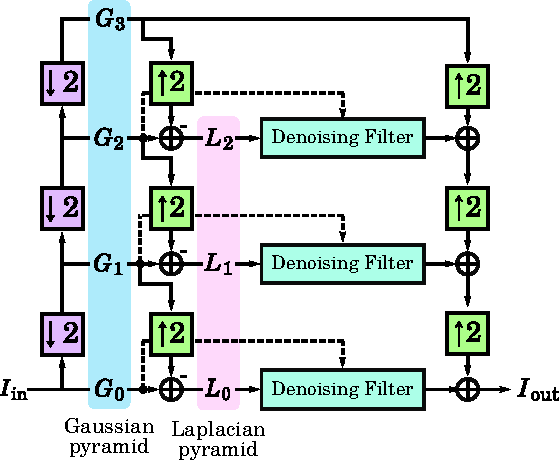
\includegraphics[scale=0.7]{figures/conventional_laplacian_pyramid.pdf}
  }
  \hspace{0.2in}
  \subfloat[Cascaded Laplacian Pyramid]{
    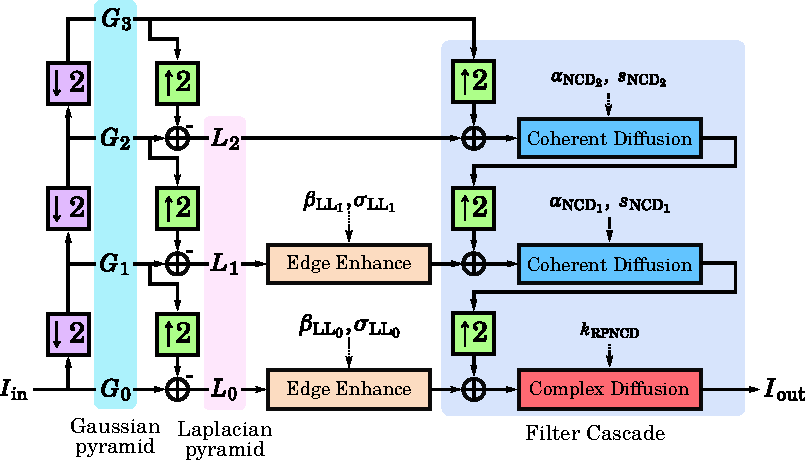
\includegraphics[scale=0.7]{figures/multiscale_filter.pdf}
  }
  \caption{Block diagram of the considered image enhancement scheme.}
\end{figure*}

\subsubsection{Local Laplacian Filters}

\cite{10.1145/2010324.1964963}


\subsubsection{Overview}


\paragraph{Diffusion Strength and Edge Detection}
While various alternative choices for determining \(\lambda_1, \lambda_2\), have been proposed over the years, most of them require some form of edge detection.
Therefore, accurate edge-detection must be performed \textit{before} we perform speckle reduction, which is particularly challenging.
In the case of NCD, \(\kappa = {(\mu_1 - \mu_2)}^2\) acts as an edge detector which provides a good cost-performance tradeoff when used as a primary edge-detector for speckle reduction.

While some alternatives have been introduced over the years, they either provided a poor cost-performance benefit, or turned out to be system dependent.
For example, Yu et al.~\cite{yu_ultrasound_2010} proposed to use the smallest univalue segment assimilating nucleus (SUSAN,~\cite{smith_susan_1997}) edge detector while Mei et al.~\cite{mei_phase_2020} proposed to use phase assymetry (PAS,~\cite{kovesi_image_1999}).
While SUSAN is very robust, it requires large computation windows which harms its cost-performance benefits.
On the other hand, the PAS detector showed excellent results on the data used by Mei et al., but performed poorly on the data that we used for this study.
This suggests that PAS is highly dependent on the properties of the ultrasound system it is applied.


\subsubsection{Combining RPNCD and NCD}
While RPNCD has yet been applied to ultrasound images, it exhibits good fine-graded speckle reduction properties.
However, it cannot enhance the spatial coherence.


While using the eigenvectors of the structure tensor improves spatial coherence, it is still succeptible to textured speckle patterns.
This is shown in~\cref{fig:ncd_liver}, where we can see that the image processed with NCD exhibits flow-like artifacts.
Therefore, naively applying 

We will later combine both NCD and RPNCD, so that we can achieve both structure 


\begin{figure}[H]
  \centering
  \subfloat[Original]{
    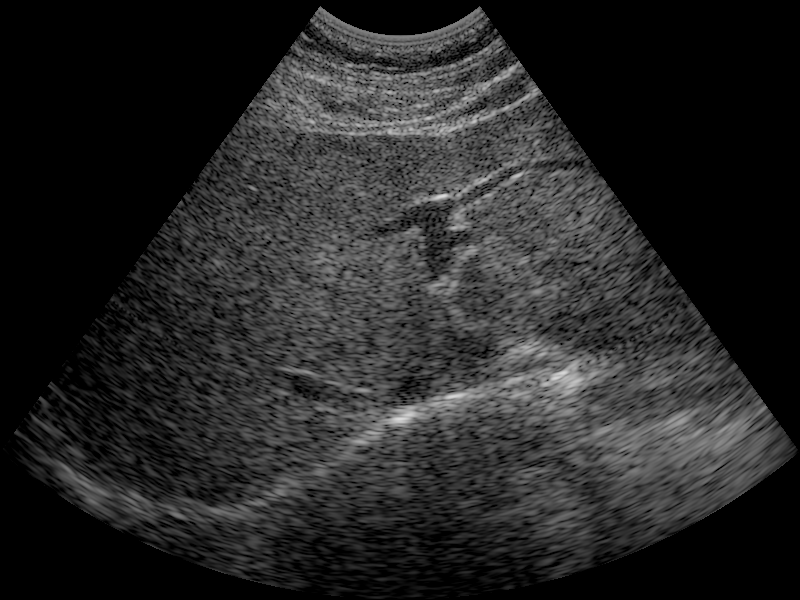
\includegraphics[trim={10cm, 10cm, 12cm, 5cm}, clip, scale=0.3]{figures/ncd_liver1.png}
  }
  \subfloat[NCD]{
    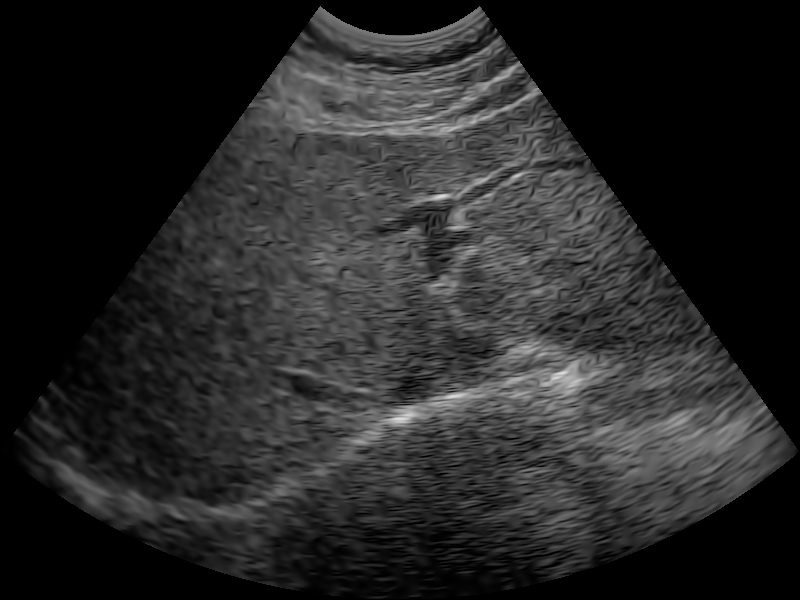
\includegraphics[trim={10cm, 10cm, 12cm, 5cm}, clip, scale=0.3]{figures/ncd_liver2.png}
  }
  \subfloat[RPNCD]{
    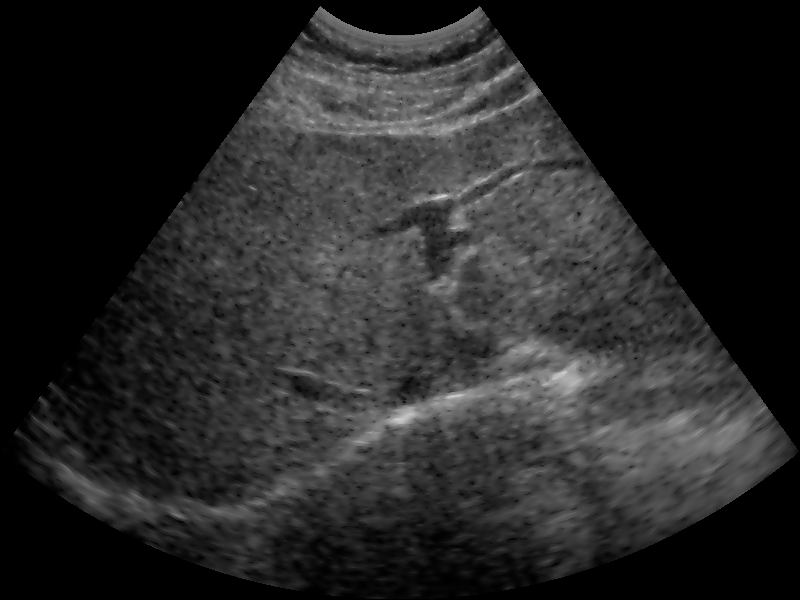
\includegraphics[trim={10cm, 10cm, 12cm, 5cm}, clip, scale=0.3]{figures/rpncd_liver.png}
  }
  \caption{Example of a liver image processed with NCD.
    The textured speckle patterns result in flow-like artifacts.}\label{fig:ncd_liver}
\end{figure}


When combined with multiscale methods, the structure matrix 



%%% Local Variables:
%%% TeX-master: "master"
%%% End:
